\section{Methodology}

\subsection{Echo State Networks}
An ``echo state network'' (also
called a ``liquid state machine'' \cite{lukosevicius_practical_2012}) is a type
of recurrent neural network that uses a single layer of many neurons called a
``reservoir''. The reservoir has an adjacency matrix $\bm{A}$ that is
\begin{enumerate}
	\item sparsely populated
	\item connected by uniformly random weights centered at zero
	\item has a large number of neurons
\end{enumerate}
A reservoir computer also satisfies the \textit{echo state property}
\cite{pathak_model-free_2018, lukosevicius_reservoir_2009}. This
property ensures that a system's state has a decaying influence on future states
(like an echo of sound or ripples on water). This property is satisfied in most
cases when the spectral radius (the absolute value of the greatest eigenvalue of
$\bm{A}$)\cite{lukosevicius_reservoir_2009} is,
\begin{align}
	\rho(\bm{A}) < 1.
\end{align}
However, the echo state property can still be satisfied for a spectral radius
greater than unity \cite{lukosevicius_practical_2012}.

\begin{figure}[H]
	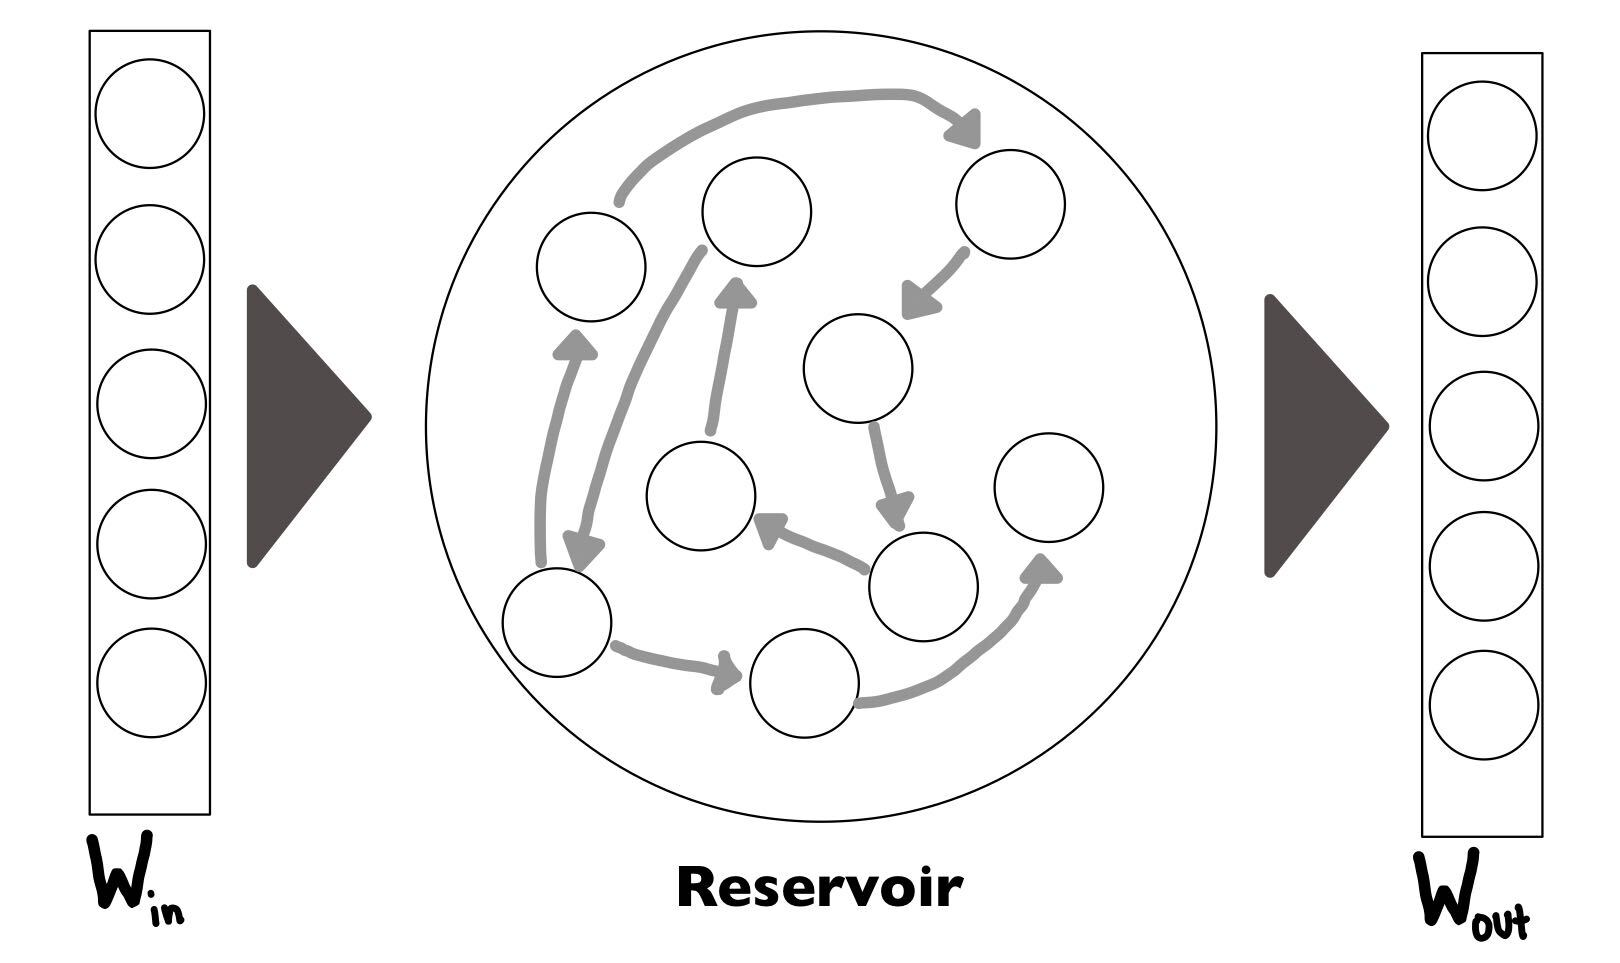
\includegraphics[width=\columnwidth]{reservoir_network.jpg}
	\caption{A basic reservoir computer or echo state network. The connections in
	the reservoir are given by $\bm{A}$}
	\label{fig:RCmodel}
\end{figure}

Figure \ref{fig:RCmodel} gives a visual representation of a basic
\acrshort{ESN}. An
input vector of length \textit{K} is mapped to the reservoir layer by an input
weight matrix $\bm{W_{in}}$. The state of the reservoir is mapped to an output
layer of length \textit{N} with an output weight matrix $\bm{W_{out}}$. An ESN
does not require $K=N$, nor does it require $K \neq N$. In this
work, the input vector is a function of time, $\bm{u}(t)$, and the output
vector is the next state of the system, $\bm{u}_p(t+\Delta t)$. Ideally, the
difference between the prediction, $\bm{u}_p$, and the actual, $\bm{u}_a$, is
minimized. During training, the output weight matrix is trained through
backpropagation using a loss function like cross entropy
\cite{pathak_model-free_2018, vlachas_backpropagation_2020}.

\subsection{Hyperparameter Search}
Due to the architecture of \acrshort{ESN}s, the weights and connections
inside the reservoir do not need to be trained and, in our choice of
implementation, cannot be. This dramatically reduces the training time because
only the linear output layer needs to be trained. One drawback of this approach
is its sensitivity to hyperparameters, which must be carefully chosen before
running the network \cite{ pathak_model-free_2018,
lukosevicius_practical_2012, lukosevicius_reservoir_2009,gallicchio_deep_2019}.
Here, we perform grid searches
to establish which combination of hyperparameters minimizes the mean squared
error of the model,
\begin{align}
	MSE &= \frac{1}{N}\sum_i^N (\hat{y} - y_i)^2\\
	\intertext{where}
	\hat{y} &= \mbox{the average value of the ouput.}\nonumber
\end{align}

\subsection{Model Prediction}
The weights of the output layer, $\bm{W_{out}}$, are
trained through backpropagation by minimizing the error. When a trained model
is given some initial state and then makes a prediction, $\bm{u}_p(t+\Delta
t)$, this prediction becomes the initial state for the next prediction and so
on. Even a good model, like in Pathak et. al \cite{pathak_model-free_2018}, has
some propagating error that deteriorates the prediction fidelity.
